\scanpage{55}
\mspage{\handwritten{23}\,\raisebox{.6ex}{\begin{tikzpicture}[x=1cm,y=1cm,baseline=0pt]\fill (0,0) circle (.018);\end{tikzpicture}}}
% archive sheet number: 54

$\handwritten{\rho}(e_{\unsure{o|0}})=\handwritten{\sum}a_i\handwritten{\otimes}e_i$ shows that $\handwritten{\sum\Delta}(a_i)\handwritten{\otimes}e_i=\handwritten{\sum}a_i\handwritten{\otimes\rho}(e_i)=\handwritten{\sum}a_i\handwritten{\otimes}a_j^i\handwritten{\otimes}e_j$, from which one de-\linebreak duces that $\handwritten{\Delta}(a_i)=a_{\unsure{o|0}}\handwritten{\otimes}a_i++\handwritten{\sum_{j\geqslant1}}a_j\handwritten{\otimes}a_i^j$; therefore, since for $j\geqslant1$, $a_j\in I$, one sees that $q\mathbin{o}\handwritten{\Delta}(a_i)=p(a_{\unsure{o|0}})\handwritten{\otimes}a_i$, so that \unsure{for|poue} $1\leqq i\leqq n$, $a_i$ is semi-invariant under $H$ \deleted{of invara} \deleted{of invariant}\inserted{\handwritten{of weight}} $p(a_{\unsure{o|0}})$, independent of $i$; \deleted{therefore all the $a_i$ are semi-invariant under $H$ with the same associated char-\linebreak acter, therefore of the same weight. Finally}\inserted{\handwritten{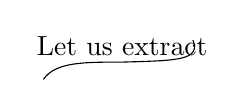
\begin{tikzpicture}[x=1cm,y=1cm,baseline=(n.base)]\node (n) at (0,0) {Let us extract};\draw (-1.0,-.42) .. controls (-.85,-.2) and (-.5,-.2) .. (0,-.2) .. controls (.7,-.18) and (1,-.18) .. (.9,.08);\end{tikzpicture}}} \unsure{from the|dy} system $(a_1,\ldots,a_n)$, \deleted{one can extract} a maximal system of linearly independent vect\deleted{\unsure{or}}\handwritten{\unsure{or}}s, which one may suppose is denoted $(a_{\handwritten{1}},\mathinner{..},a_m)$. \inserted{\handwritten{Then the $a_i$, $i=1,\mathinner{-\,-},m$ are linearly \unsure{independent|independent|independent}), semi invariant under $H$, and of the same weight.}}

Conversely, let $H'$ be a closed subgroup prescheme of $G$ under which each of the $a_i$ $(1\leqq i\leqq m)$ is semi-invariant. \inserted{\handwritten{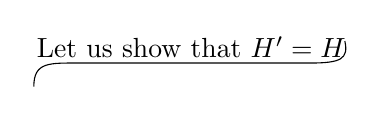
\begin{tikzpicture}[x=1cm,y=1cm,baseline=(n.base)]\node (n) at (0,0) {Let us show that $H'=H$};\draw (-2,-.5) .. controls (-2,-.18) and (-1.8,-.2) .. (-1.4,-.2)--(1.5,-.2) .. controls (1.9,-.2) and (2,-.15) .. (1.95,.08);\end{tikzpicture}}} There likewise exists an ideal $I'$ of $A$ such that the algebra $B'$ of $H'$ is isomorphic to $A/I'$; let us write $p':A\handwritten{\longrightarrow}A/I'$ for the canonical map, and $q'=p'\handwritten{\otimes}\operatorname{id}_A$. By hypothesis, for $1\leqq i\leqq m$, there exists $\handwritten{\lambda}_i\in B'$ such that $q'\mathbin{o}\handwritten{\Delta}(a_i)=\handwritten{\sum}p'(a_j)\handwritten{\otimes}a_i^j=\handwritten{\lambda}_i\handwritten{\otimes}a_i$. Now axiom (CM2) of (\deleted{Exp}I 4.7\handwritten{\unsure{;|.}}2) shows that $e_i=\handwritten{\sum\eta}(a_j^i)e_j$, hence that $\handwritten{\eta}(a_j^i)=\handwritten{\delta}_{ij}$ (Kronecker symbol); the equality $\handwritten{\sum}p'(a_j)\handwritten{\otimes\eta}(a_j^i)=\handwritten{\lambda}_i\handwritten{\otimes\eta}(a_i)$ therefore reads $p'(a_i)=0$ for $1\leqq i\leqq m$, since $\handwritten{\eta}(a_i)\handwritten{=\eta}(a_i^{\unsure{o|0}})=0$ for $1\leqq i\leqq m$; consequently, one has $a_i\in I'$ for $1\leqq i\leqq m$, so that $a_i\in I'$ for $1\leqq i\leqq n$. Thus, if one sets $\handwritten{\sigma}'=(p'\handwritten{\otimes}\operatorname{id}_E)\mathbin{o}\handwritten{\Delta}$, $\handwritten{\sigma}'(e_{\unsure{o|0}})=\handwritten{\sum}p'(a_i)\handwritten{\otimes}e_i$ is proportional to $e_{\unsure{o|0}}$, so that $q'\mathbin{o}\handwritten{\Delta}(W)\subset A/I'\handwritten{\otimes}_k W$, in other words that $W$ is stable under $H'$. Since $W$ generates\inserted{\handwritten{
\begin{tikzpicture}[x=1cm,y=1cm,baseline=(n.base)]\node (n) at (0,0) {the ideal};\draw (-.75,-.15) .. controls (-.5,-.1) and (-.2,-.3) .. (-.1,-.5) .. controls (.05,-.1) and (.6,-.35) .. (.75,.02);\end{tikzpicture}}} $I$, $I$ is stable under $H'$, hence $q'\mathbin{o}\handwritten{\Delta}(I)\subset(A/I')\handwritten{\otimes}_k I$, and $q'\mathbin{o}\handwritten{\Delta}$ defines by passage to the quotient a linear map $A/I\handwritten{\longrightarrow}(A/I')\handwritten{\otimes}_k(A/I)\handwritten{=((A/I')\otimes_k A)/((A/I')\otimes_k I)}$ hence \deleted{\illegible{14}}\inserted{the restriction to $H'\handwritten{\times_{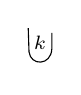
\begin{tikzpicture}[x=1cm,y=1cm,baseline=(n.base)]\node[inner sep=0pt] (n) at (0,0) {\scriptsize $k$};\draw (-.15,.18)--(-.14,-.12) .. controls (-.12,-.3) and (.14,-.3) .. (.15,-.08)--(.15,.12);\end{tikzpicture}}}H$ of the multiplication morphism of $G$ factors through $H$}, which implies that $H'$ is \deleted{con-\linebreak tained in $H$, \unsure{q.e.d.}} a subgroup prescheme of $H$, q.e.d.

\margin{\handwritten{\unsure{There must exist} \unsure{a} \unsure{reference|reference} \unsure{here} \unsure{Exp.} $\mathrm{VI}_{\unsure{A|a}}$ (\unsure{see the end}) \\ \unsure{I have|I write} \illegible{3} \unsure{in} \illegible{2} \unsure{elementary|proof}}}
\uline{Theorem} 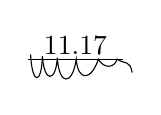
\begin{tikzpicture}[x=1cm,y=1cm,baseline=(n.base)]\node (n) at (0,0) {\handwritten{11.17}};\draw (-.6,-.17)--(.6,-.17);\draw[thin] (-.57,-.11) .. controls (-.55,-.5) and (-.43,-.5) .. (-.42,-.13);\draw (-.42,-.13) .. controls (-.4,-.47) and (-.25,-.47) .. (-.23,-.15) .. controls (-.21,-.51) and (-.04,-.51) .. (.01,-.17) .. controls (.03,-.45) and (.2,-.45) .. (.29,-.17) .. controls (.36,-.29) and (.49,-.29) .. (.53,-.17) .. controls (.64,-.24) and (.69,-.18) .. (.72,-.34);\end{tikzpicture} (Chevalley).- Let $k$ be a field, $G$ an affine $k$-group (not necessarily al\unsure{-|.}\linebreak gebraic), and $H$ a closed subgroup prescheme of $G$ \uline{invariant} in $G$; then the quotient sheaf (for the fpqc topology) $G/H$ is representable by an \uline{affine} $k$-group.

\margin{\figure{\handwritten{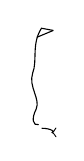
\begin{tikzpicture}[x=0.35cm,y=0.35cm]
\draw[thin] (0.45,3.5)--(-.15,3.25);\draw[thin] (0.45,3.5) -- (0.02,3.58) .. controls (-0.35,3.0) and (-0.12,2.4) .. (-0.30,1.95) .. controls (-0.46,1.45) and (-0.01,1.03) .. (-0.17,0.65) .. controls (-0.35,0.30) and (-0.30,0.03) .. (-0.08,0.08);
\draw[thin,->] (0.03,-0.05) .. controls (0.40,-0.05) and (0.52,-0.20) .. (0.38,-0.20);
\end{tikzpicture}}}}
\uline{First case} : \deleted{s}\inserted{\handwritten{S}}uppose first that $G$ is algebraic. According to (\deleted{Exp.} $\mathrm{VI}_A$ 3.2), the cokernel $K$ of the injec-\linebreak tion $H\handwritten{\longrightarrow}G$ exists, \deleted{and} the canonical morphism $p:G\handwritten{\longrightarrow}K$ is \deleted{faithfully flat , and quasi-com-\linebreak pact, since $G$ is of finite type over $k$, and $K$, which is equipped with a $k$-group structure (Exp. $\mathrm{VI}_A$ 5.2) is separated over $k$ (Exp. $\mathrm{VI}_A$ 0.2). Thus $p$ is} covering for the fpqc topology, \deleted{so \deleted{\unsure{u}} (\deleted{\unsure{Exp.}} IV 4.4.3) that}\inserted{\handwritten{and}} $K$ represents the quptient sheaf $G/H$ for the fpqc topology;
\figure{\handwritten{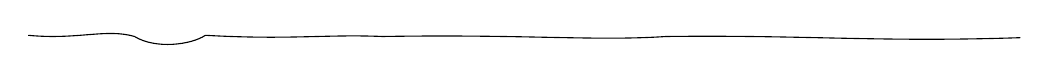
\begin{tikzpicture}[x=.9cm,y=.3cm]\draw[thin] (0,.1) .. controls (.7,-.1) and (1.1,.4) .. (1.5,.05) .. controls (1.8,-.5) and (2.3,-.3) .. (2.5,.1) .. controls (3.7,-.1) and (4.2,.15) .. (5,.05) .. controls (7,.15) and (8,-.15) .. (9,.05) .. controls (11,.12) and (12,-.2) .. (14,0);\end{tikzpicture}}}
